\begin{fullwidth}
\chapter{\label{ch:super_syllables}
Experimental results}
\end{fullwidth}

\begin{chabstract}

In this chapter we report subjects behavioral performance ...

\end{chabstract}


\section{Behavioral performance}
%
The subjects had a behavioral performance above 97\% in both visual and auditory \emph{Pseudoword matching tasks}, except for \emph{Subject 05} that reported concentration span issues over all the acquisition.
Note that due to the experimental design structure, in which we only query few random samples, small score decrements can imply distraction over an important task segment.
\emph{Subjects 01 and 04} reported in the second auditory session that the volume was not high enough to be comfortable, although this did not reflect on their behavioral performance.
So we consider all subjects data apt to neuroimaging interpretation, with caution over \emph{Subject 05}. Behavioral performance details are provided in Table \ref{table:behavior}.


\begin{table}
\begin{tabular}{|>{\bfseries}l|rrr|}
\toprule
Subject &  Visual (\%) &  Auditory (\%) &  Overall (\%) \\
\midrule
01 &        97.22 &          97.22 &    97.22 \\
02 &       100.00 &          98.61 &    99.31 \\
03 &        97.92 &          97.22 &    97.57 \\
04 &        99.31 &          99.31 &    99.31 \\
05 &        92.36 &          88.89 &    90.62 \\
\bottomrule
\end{tabular}
\caption{\textbf{Behavioral performance on \emph{Pseudoword matching task}:} Performance correspond to correct answers to the same or different query, where no answer is considered as incorrect. Visual and Auditory headers refer to the sensory modality of the task, where overall is the mean performance of both modalities.}
\label{table:behavior}
\end{table}


\section{Sanity checks}\label{sec:sanity_checks}

\paragraph{Language localizer activations:}
The contours of the language localizers' contrasts, thresholded at p-value < 0.001, for both auditory and visual modalities are presented in Figure \ref{fig:language_localizers} for all subjects.


We appreciate a variability between the modalities, that particularly disfavors activations of the visual one, in which the subjects can get distracted from perceiving and processing the stimuli more easily, than in the auditory case.
This could also be expected from the intrinsic variability of different experimental designs in language localizers as demonstrated by Mahowald et al. \citep{mahowald2016reliable}.
Nonetheless, there is good spatial agreement between the activation regions of visual and auditory modalities, portraying a left lateralized network that covers the fronto-temporal language system that has been well depicted in previous imaging studies\citep{mahowald2016reliable, fedorenko2010new, dehaene2010learning, binder1997human}.


Note that \emph{Subject 5}, who reported concentration problems, have the weakest language network activation from all subjects, which can hinder importantly our capacity to interpret his language related classification results.


\begin{figure*}[ht]
\scriptsize
\hspace{-4ex}
\begin{tabular}{ccc}
\textbf{\Large Subject 1} & \textbf{\Large Subject 2} & \textbf{\Large Subject 3}\\
{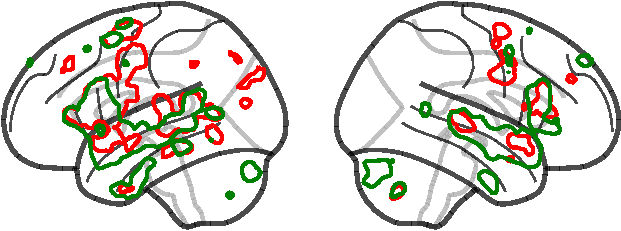
\includegraphics[width=.33\linewidth]{figures/part_II/langloc_01.pdf}}
\hspace{-1ex}
&{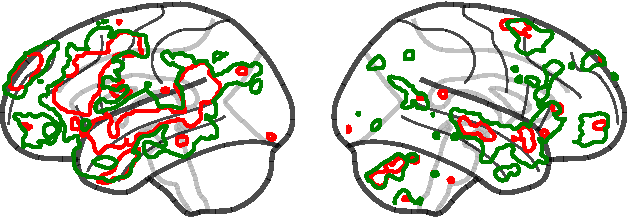
\includegraphics[width=.33\linewidth]{figures/part_II/langloc_03.pdf}}
\hspace{-1ex}
&{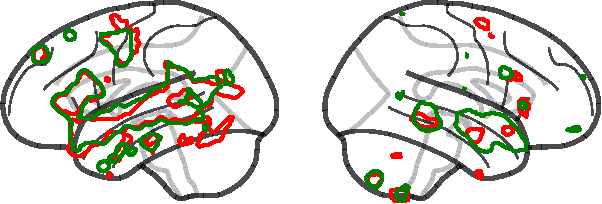
\includegraphics[width=.33\linewidth]{figures/part_II/langloc_04.pdf}}
\hspace{-1ex}\\
\rule{0pt}{6ex}
\textbf{\Large Subject 4} & \textbf{\Large Subject 5} & {}\\
{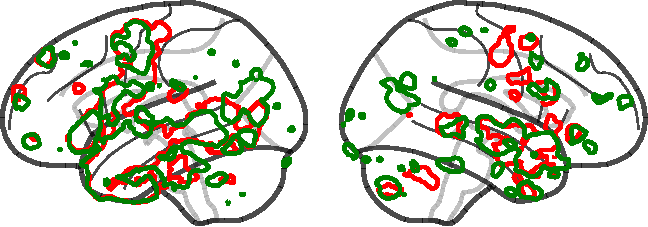
\includegraphics[width=.33\linewidth]{figures/part_II/langloc_05.pdf}}
\hspace{-1ex}
&{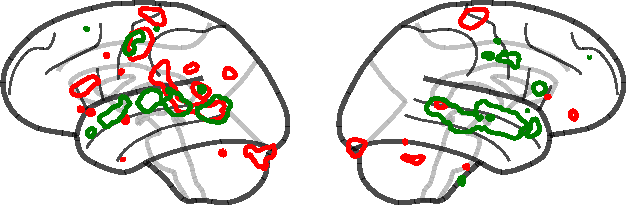
\includegraphics[width=.33\linewidth]{figures/part_II/langloc_06.pdf}}
\hspace{-1ex}
&{
\includegraphics[width=.2\linewidth]{figures/part_II/langloc_legend.pdf}}
\hspace{-1ex} \\
\end{tabular}
\vspace{3ex}
\caption{\textbf{Language localizers:} We show left and right hemispheric contours of the language localizer contrast of normal phrases over consonant strings, thresholded at a p-value < 0.0001.
We present in red the contrast from the visual modality and in green the contrast from the auditory modality. Statistical images correspond to the anatomical space of each subject.}
\label{fig:language_localizers}
\end{figure*}

Checking that our language localizers agree with Fedorenko regions...






\paragraph{Motor activations:}
We verified the integrity of the activation maps of the \emph{Pseudoword matching task} with statistical tests portraying the left and right hand button press contrast and retinotopic effects of syllable position.
These tests were also useful to verify the capacity of Support Vector Classification (SVC), with the default hyper-parameters provided in the Nilearn\citep{abraham2014machine} codebase, to decode the condition beta maps.

\begin{figure*}[hb]
\scriptsize
\hspace{-4ex}
\begin{tabular}{cccccl}
\textbf{\Large Subject 1} & \textbf{\Large Subject 2} & \textbf{\Large Subject 3} & \textbf{\Large Subject 4} & \textbf{\Large Subject 5} & {}\\
{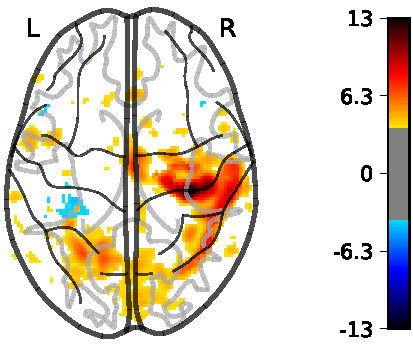
\includegraphics[width=.14\linewidth]{figures/part_II/press_vis_01.pdf}}
\hspace{1ex}
&{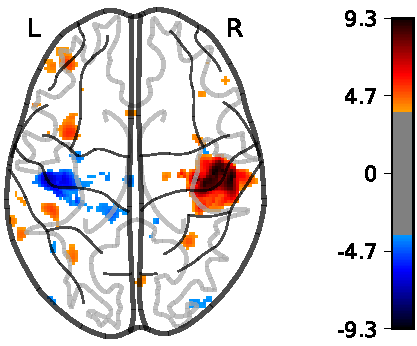
\includegraphics[width=.14\linewidth]{figures/part_II/press_vis_03.pdf}}
\hspace{1ex}
&{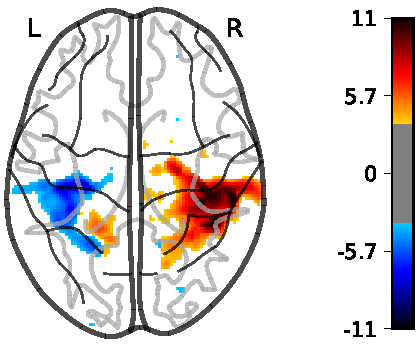
\includegraphics[width=.14\linewidth]{figures/part_II/press_vis_04.pdf}}
\hspace{1ex}
&{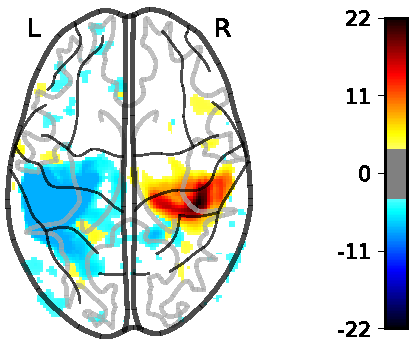
\includegraphics[width=.14\linewidth]{figures/part_II/press_vis_05.pdf}}
\hspace{1ex}
&{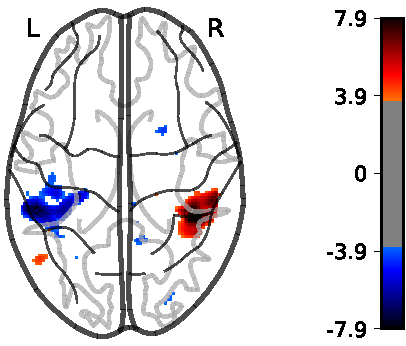
\includegraphics[width=.14\linewidth]{figures/part_II/press_vis_06.pdf}}
\hspace{1ex}
& {} \\
{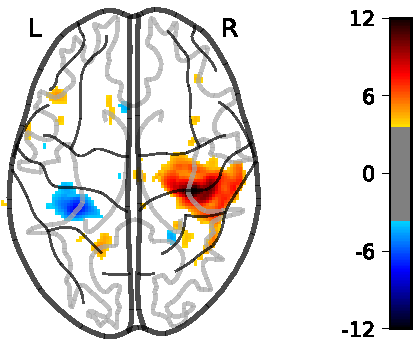
\includegraphics[width=.14\linewidth]{figures/part_II/press_aud_01.pdf}}
\hspace{1ex}
&{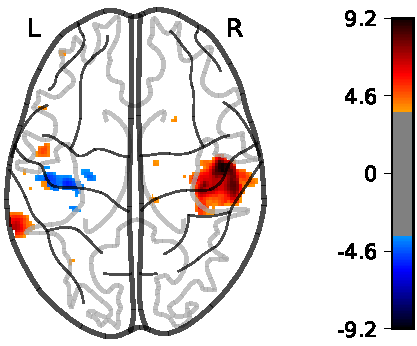
\includegraphics[width=.14\linewidth]{figures/part_II/press_aud_03.pdf}}
\hspace{1ex}
&{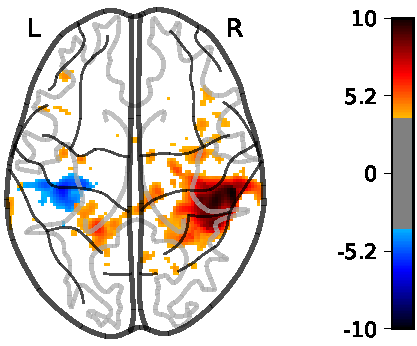
\includegraphics[width=.14\linewidth]{figures/part_II/press_aud_04.pdf}}
\hspace{1ex}
&{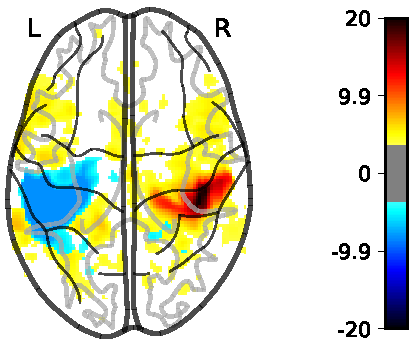
\includegraphics[width=.14\linewidth]{figures/part_II/press_aud_05.pdf}}
\hspace{1ex}
&{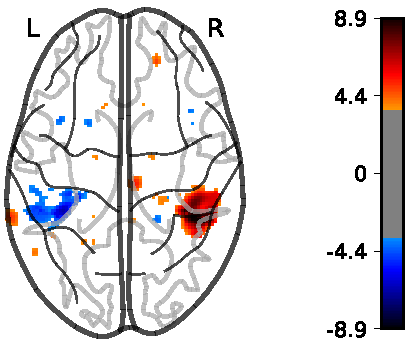
\includegraphics[width=.14\linewidth]{figures/part_II/press_aud_06.pdf}}
\hspace{1ex}
&{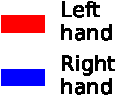
\includegraphics[width=.10\linewidth]{figures/part_II/press_legend.pdf}} \\
\end{tabular}
\vspace{3ex}
\caption{\textbf{Button press effects:} We show the left button press over right button press contrast Z scores from the auditory modality, thresholded at p < 0.0001, for all subjects. Statistical images correspond to the anatomical space of each subject.}
\label{fig:button_press}
\end{figure*}


We verified that we can classify the left and right button press beta maps derived from the \emph{Pseudoword matching task} General Linear Model (GLM), alongside the pseudoword condition maps, as explained in the methods section \ref{sec:processing}.
Z score maps of the left over right button press contrast, for all subjects, are shown in Figure \ref{fig:button_press}, confirming a good statistical separation of hand responses in the \emph{Pseudoword matching task}.
As can be seen in Table \ref{table:clic}, we achieve high classification scores of right and left button press events for all subjects.
Moreover as would be expected, the classification generalize across sensory modalities.


\begin{table}
\begin{tabular}{|>{\bfseries}l|rrrrr|}
\toprule
(Train, Test) & (V, V) & (A, A) & (V, A) & (A, V) & (V-A, V-A) \\
Subject & (\%) &  (\%)   & (\%)  & (\%)  &   (\%)\\
\midrule
01      &   84.38*** &   93.50*** &   80.84*** &   76.94*** &           90.88*** \\
02      &   95.38*** &   92.50*** &   84.03*** &   93.03*** &           95.31*** \\
03      &   98.00*** &   99.00*** &   93.91*** &   98.75*** &          100.00*** \\
04      &   97.38*** &   99.50*** &   97.50*** &   98.72*** &          100.00*** \\
05      &   86.62*** &   77.62*** &   90.12*** &   74.28*** &           93.56*** \\
\bottomrule
\end{tabular}
\vspace{4ex}
\caption{\textbf{Classification of left and right button press maps of \emph{Pseudoword matching task}:} \emph{V} corresponds to the Visual modality and \emph{A} to the Auditory modality. \emph{V-A} corresponds to pooling together both datasets for training and testing.}
\label{table:clic}
\end{table}

\blankfootnote{\emph{chance: 50\% \\ * : p < 0.01,\\ ** : p < 0.001,\\ *** : p < 0.0001 \\ Bonferroni corrected for 25 similar tests performed}}

\paragraph{Visual activations:}
Then we visually verified the statistical effects of left and right syllable position in the Visual hOc1 region.
In the experimental design we asked the subjects to fixate a centered green dot before stimuli presentation.
So we expected, from well known retinotopic effects in the primary visual cortex \citep{tootell1998retinotopy}, to see an hemispheric partition of left and right syllable position effects, such that left syllable effects would be emphasized in the right hemisphere and right syllable effects in the left hemisphere.
This was the case, as can be seen in Figure \ref{fig:retinotopy}, where \emph{Subjects 1 and 4} have the clearest retinotopic activations.
Nonetheless we can also appreciate in the images that some subjects did not manage to completely follow the fixation instruction, since effects of both positions are present together in both hemispheres.


\begin{figure*}[ht]
\scriptsize
\vspace{5ex}
\hspace{-4ex}
\begin{tabular}{cccccl}
\textbf{\Large Subject 1} & \textbf{\Large Subject 2} & \textbf{\Large Subject 3} & \textbf{\Large Subject 4} & \textbf{\Large Subject 5} & {}\\
{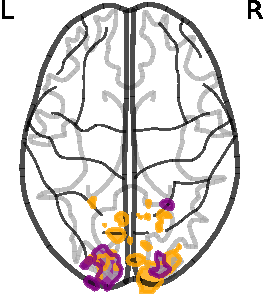
\includegraphics[width=.14\linewidth]{figures/part_II/retinotopy_01.pdf}}
\hspace{1ex}
&{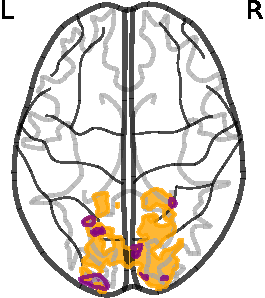
\includegraphics[width=.14\linewidth]{figures/part_II/retinotopy_03.pdf}}
\hspace{1ex}
&{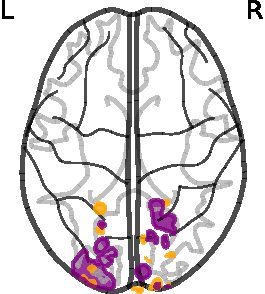
\includegraphics[width=.14\linewidth]{figures/part_II/retinotopy_04.pdf}}
\hspace{1ex}
&{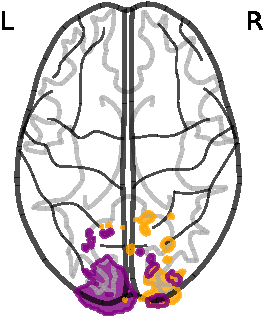
\includegraphics[width=.14\linewidth]{figures/part_II/retinotopy_05.pdf}}
\hspace{1ex}
&{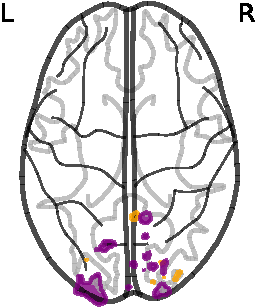
\includegraphics[width=.14\linewidth]{figures/part_II/retinotopy_06.pdf}}
\hspace{1ex}
&{
\includegraphics[width=.12\linewidth]{figures/part_II/retinotopy_legend.pdf}}
\hspace{-1ex} \\
\end{tabular}
\vspace{3ex}
\caption{\textbf{Retinotopy effect:} We show first and second syllable effects masked by the Visual hOc1 region, thresholded at a p-value < 0.005.
We present in orange the effect of first position and in purple the effect of second position. Statistical images correspond to the anatomical space of each subject.}
\label{fig:retinotopy}
\end{figure*}


\section{Sensory representations}

Considering we have included in our design an auditory and visual modality, it is interesting to first explore how the different classification models capture bi-syllabic representations in the primary visual and auditory regions presented in section \ref{sec:subject_networks}.

The regions of the Amuntz atlas are importantly sized and might overlap with the language network, so to make sure any captured effect can be interpreted only as sensory, we intersected these regions\footnote{Visual hOc1 and Auditory Te10} with the non language gray matter section that showed any effects of position or interaction, in a similar way to how the language searchlight region was defined.


Comment on the peripheral auditory prediction on visual activations. \ref{fig:visual_amodal}

\begin{figure}[ht]
\scriptsize
\vspace{5ex}
\hspace{-4ex}
\begin{tabular}{ccc}
\textbf{\Large Visual} & \textbf{\Large Auditory} & \textbf{\Large Amodal}\\
{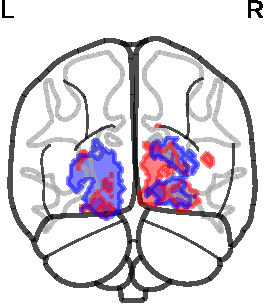
\includegraphics[width=.18\linewidth]{figures/part_II/searchlight/amodal/visual_Vis-Vis_segmentation.pdf}}
\hspace{1ex}
&{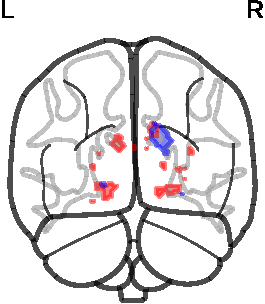
\includegraphics[width=.18\linewidth]{figures/part_II/searchlight/amodal/visual_Aud-Aud_segmentation.pdf}}
\hspace{1ex}
&{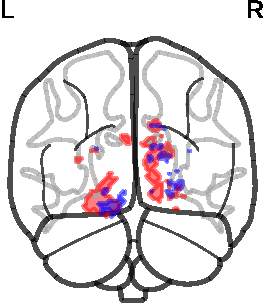
\includegraphics[width=.18\linewidth]{figures/part_II/searchlight/amodal/visual_amodal_segmentation.pdf}}
\hspace{1ex}\\
\end{tabular}
\vspace{3ex}
\caption{\textbf{modality specific models in visual region:} We compare results from the visual and auditory datasets, alongside the amodal prediction (significant cross modal classification from both modalities to each other (signficant when train in Vis and predicting Aud and when trained in Aud and predicting Vis))}
\label{fig:visual_amodal}
\end{figure}


Then we emphasize classification of the visual modality in the visual region \ref{fig:visual_searchlight}

% would adding a confusion matrix to depict first and second position classification difficulties be interesting? then to compare it with those from the auditory modality. Initial inspection of visual models revealed particular difficulty with one of the syllables.

In the case of the visual modality, due to the retinotopic effects shown in the previous section \ref{sec:sanity_checks}, 
we would expect to obtain significant classification scores for the separate models of first and second syllable. Develop this in more detail, maybe add a table of a cluster?


\begin{figure*}[ht]
\scriptsize
\hspace{-4ex}
\begin{tabular}{ccc}
\textbf{\Large First vs Second syllable} & \textbf{\Large Distributed (First and Second)}\\
{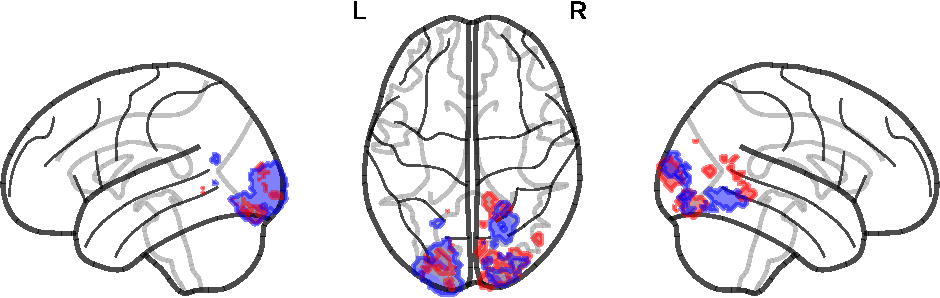
\includegraphics[width=.4\linewidth]{figures/part_II/searchlight/visual_Vis-Vis_segmentation.pdf}}
\hspace{-1ex}
&{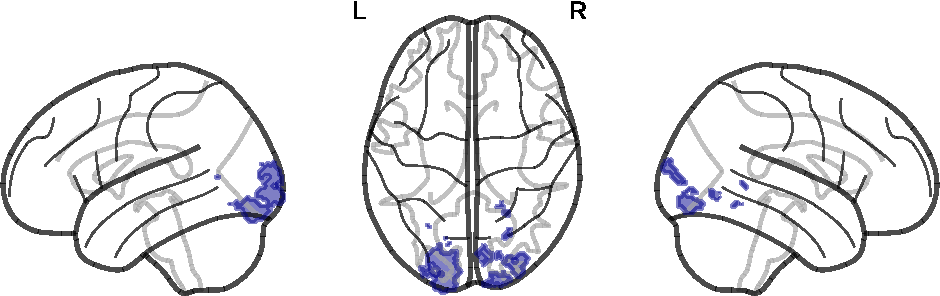
\includegraphics[width=.4\linewidth]{figures/part_II/searchlight/visual_Vis-Vis_locality.pdf}}
\hspace{-1ex}
&{\multirow{-9}{200mm}{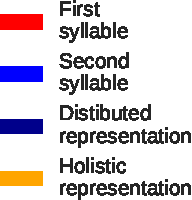
\includegraphics[width=.15\linewidth]{figures/part_II/searchlight/searchlight_legend.pdf}}}\\
%&\smash{\parbox[t]{\lwidth}{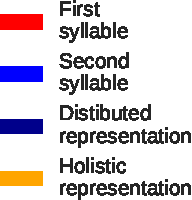
\includegraphics[width=.15\linewidth]{figures/part_II/searchlight/searchlight_legend.pdf}}}\\
\rule{0pt}{6ex}
\textbf{\Large Holistic (Syllable combination)} & {}\\
{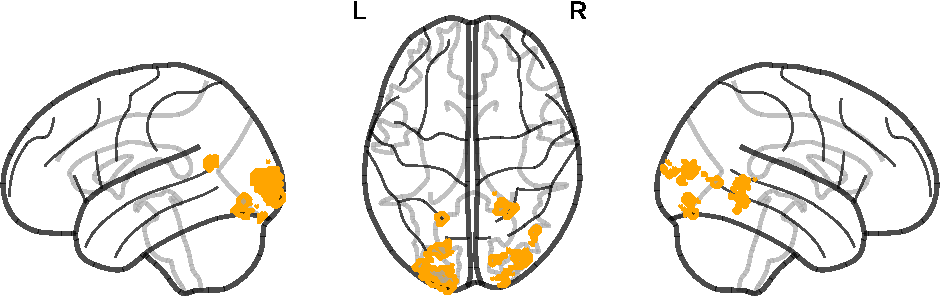
\includegraphics[width=.4\linewidth]{figures/part_II/searchlight/visual_Vis-Vis_holistic.pdf}}
\hspace{-1ex}
& {}\\
\end{tabular}
%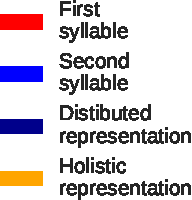
\includegraphics[width=.15\linewidth]{figures/part_II/searchlight/searchlight_legend.pdf}
\vspace{3ex}
\caption{\textbf{Visual classification models:} We present clusters of the overlapping 3 voxel dilated thresholded classification regions of at least 4 subjects. Subject classification results were thresholded above chance level and with bonferroni corrected p < 0.05. We show the overlapped clusters of the first and second syllable models, the distributed model (classification of the joint first and second position models) and the holistic model (classification of syllable combinations). The images reflect classification results in the visual modality dataset of the \emph{Pseudoword matching task}}
\label{fig:visual_searchlight}
\end{figure*}


Interesting amodal effects in auditory region, likely due to subvocalization during reading. But there are also plenty of effects from reading in auditory region according to the literature. To develop in the discussion.
\ref{fig:sensory_amodal}

\begin{figure}[ht]
\scriptsize
\vspace{5ex}
\hspace{-4ex}
\begin{tabular}{ccc}
\textbf{\Large Visual} & \textbf{\Large Auditory} & \textbf{\Large Amodal}\\
{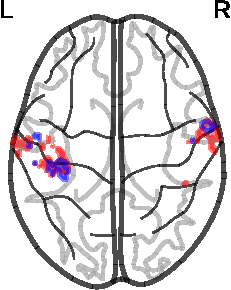
\includegraphics[width=.18\linewidth]{figures/part_II/searchlight/amodal/auditory_Vis-Vis_segmentation.pdf}}
\hspace{1ex}
&{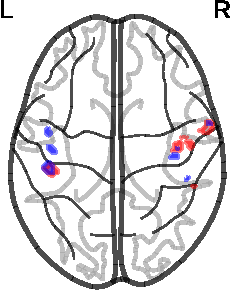
\includegraphics[width=.18\linewidth]{figures/part_II/searchlight/amodal/auditory_Aud-Aud_segmentation.pdf}}
\hspace{1ex}
&{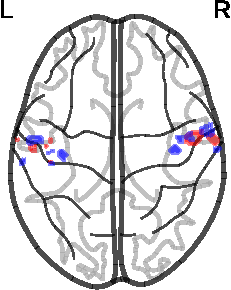
\includegraphics[width=.18\linewidth]{figures/part_II/searchlight/amodal/auditory_amodal_segmentation.pdf}}
\hspace{1ex}\\
\end{tabular}
\vspace{3ex}
\caption{\textbf{Auditory amodal representations:} We show}
\label{fig:auditory_amodal}
\end{figure}


So we present globally amodal effects in the case of the auditory modality
\ref{fig:auditory_searchlight}

Do a confusion matrix reflect the way we picked the sounds. So they are all equally misclassified. We did not really optimized the visual presentation of the syllables. Revisit paper showing distance of phonemes in auditory cortex.


\begin{figure*}[ht]
\scriptsize
\hspace{-4ex}
\begin{tabular}{ccc}
\textbf{\Large First vs Second syllable} & \textbf{\Large Distributed (First and Second)}\\
{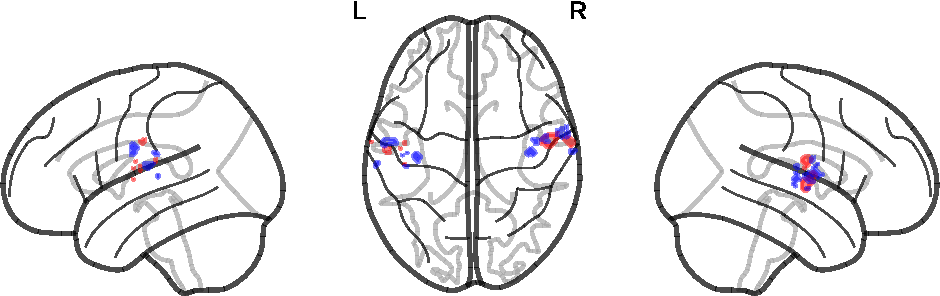
\includegraphics[width=.4\linewidth]{figures/part_II/searchlight/auditory_amodal_segmentation.pdf}}
\hspace{-1ex}
&{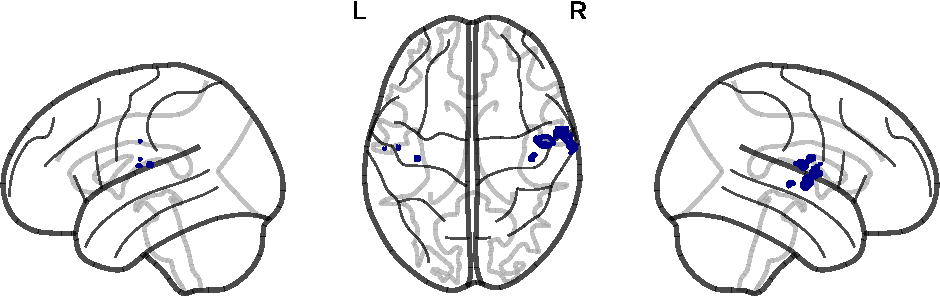
\includegraphics[width=.4\linewidth]{figures/part_II/searchlight/auditory_amodal_locality.pdf}}
\hspace{-1ex}
&{\multirow{-9}{200mm}{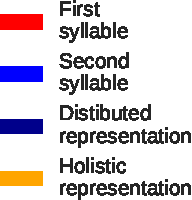
\includegraphics[width=.15\linewidth]{figures/part_II/searchlight/searchlight_legend.pdf}}}\\
%&\smash{\parbox[t]{\lwidth}{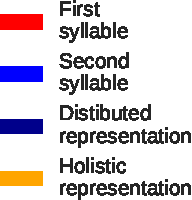
\includegraphics[width=.15\linewidth]{figures/part_II/searchlight/searchlight_legend.pdf}}}\\
\rule{0pt}{6ex}
\textbf{\Large Holistic (Syllable combination)} & {}\\
{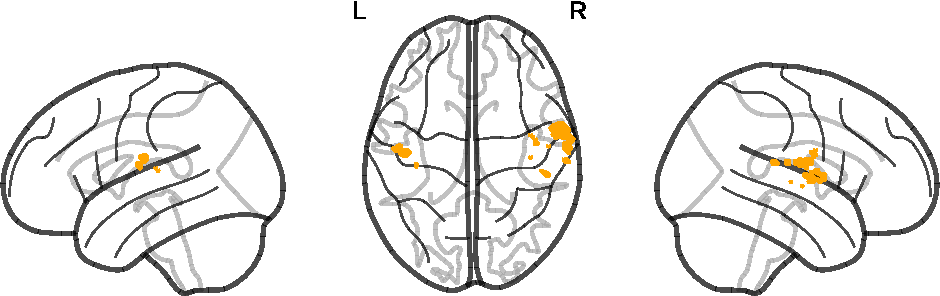
\includegraphics[width=.4\linewidth]{figures/part_II/searchlight/auditory_amodal_holistic.pdf}}
\hspace{-1ex}
& {}\\
\end{tabular}
%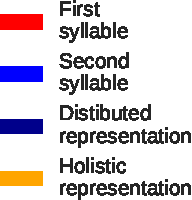
\includegraphics[width=.15\linewidth]{figures/part_II/searchlight/searchlight_legend.pdf}
\vspace{3ex}
\caption{\textbf{Auditory classification models:} }
\label{fig:auditory_searchlight}
\end{figure*}


\section{Language representations}
%notes

Show amodal effects. Interesting to us due to abstract representations.
\ref{fig:language_amodal}

\begin{figure*}[ht]
\scriptsize
\vspace{5ex}
\hspace{-4ex}
\begin{tabular}{ccc}
\textbf{\Large Visual} & \textbf{\Large Auditory} & \textbf{\Large Amodal}\\
{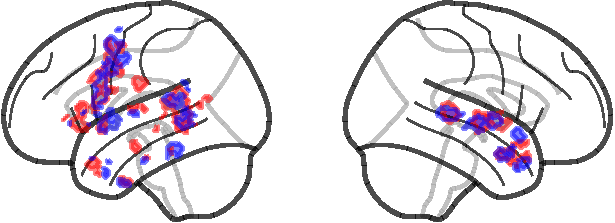
\includegraphics[width=.3\linewidth]{figures/part_II/searchlight/amodal/language_Vis-Vis_segmentation.pdf}}
\hspace{1ex}
&{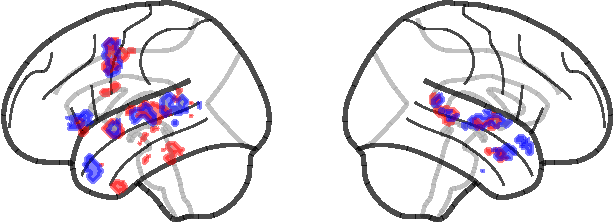
\includegraphics[width=.3\linewidth]{figures/part_II/searchlight/amodal/language_Aud-Aud_segmentation.pdf}}
\hspace{1ex}
&{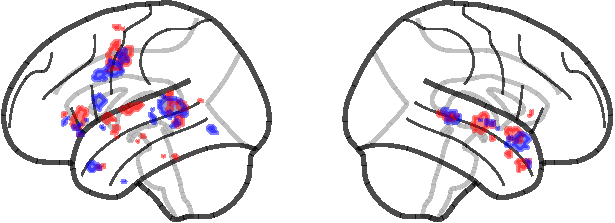
\includegraphics[width=.3\linewidth]{figures/part_II/searchlight/amodal/language_amodal_segmentation.pdf}}
\hspace{1ex}\\
\end{tabular}
\vspace{3ex}
\caption{\textbf{Language amodal representations:} We show}
\label{fig:language_amodal}
\end{figure*}


So looking for abstract representation we present amodal results. Develop on the holistic and distributed effects observed.
\ref{fig:language_searchlight}

There are broad amodal results. (many clusters survive bonferroni corrected 0.05 thresholds but look small in the plots, so we show the 0.001 uncorrected ones). We analyze amodal clusters because we are interested in abstract neural representations.

\begin{figure*}[ht]
\scriptsize
\hspace{-4ex}
\begin{tabular}{ccc}
\textbf{\Large First vs Second syllable} & \textbf{\Large Distributed (First and Second)}\\
{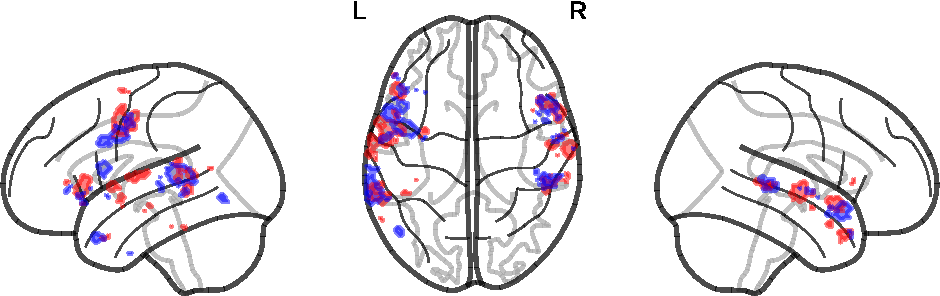
\includegraphics[width=.4\linewidth]{figures/part_II/searchlight/language_amodal_segmentation.pdf}}
\hspace{-1ex}
&{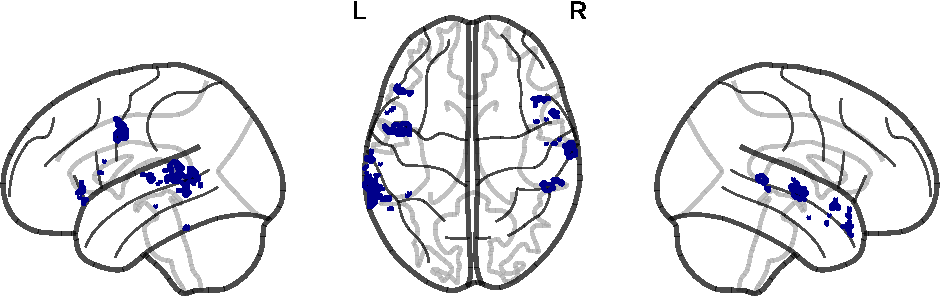
\includegraphics[width=.4\linewidth]{figures/part_II/searchlight/language_amodal_locality.pdf}}
\hspace{-1ex}
&{\multirow{-9}{200mm}{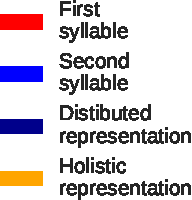
\includegraphics[width=.15\linewidth]{figures/part_II/searchlight/searchlight_legend.pdf}}}\\
%&\smash{\parbox[t]{\lwidth}{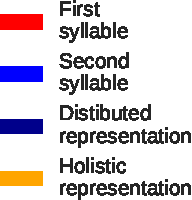
\includegraphics[width=.15\linewidth]{figures/part_II/searchlight/searchlight_legend.pdf}}}\\
\rule{0pt}{6ex}
\textbf{\Large Holistic (Syllable combination)} & {}\\
{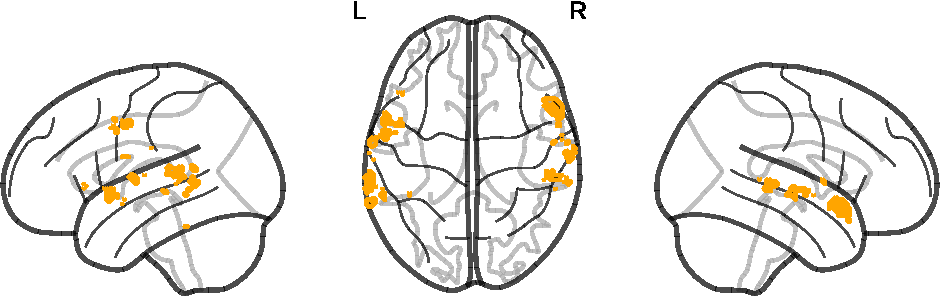
\includegraphics[width=.4\linewidth]{figures/part_II/searchlight/language_amodal_holistic.pdf}}
\hspace{-1ex}\\
\end{tabular}
%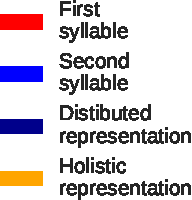
\includegraphics[width=.15\linewidth]{figures/part_II/searchlight/searchlight_legend.pdf}
\vspace{3ex}
\caption{\textbf{Language classification models:} }
\label{fig:language_searchlight}
\end{figure*}

Compare with Fedorenko classification of language localizer regions the clusters extracted.

Present tables showing the classification achieved in the biggest amodal cluster that survives correction?

possible plot of statistical interaction and effects in holistic clusters vs distributed clusters? If plenty of interactions present in distributed clusters we could give an argument for the failure of the superposition test, although this extra interaction could mean many things to be developed in the following discussion?

Show the link with previous morphological effects by checking on coordinates close to clusters. (only the ones that survive correction or all and the corrected ones emphasized?). We do this for holistic and distributed representations. Table \ref{table:holistic_effects} and Table \ref{table:distributed_effects}


\begin{table}
\begin{tabular}{llll}
\toprule
{} &       Cluster center & Cluster size &                                    Related effects \\
\midrule
0 &   [21.0, 56.0, 50.0] &           13 &                                                 [] \\
1 &   [21.0, 67.0, 55.0] &           12 &  P-over-W-Left\_superior\_temporal\_gyrus, Passiv... \\
2 &   [22.0, 84.0, 52.0] &           27 &                                                 [] \\
3 &   [27.0, 94.0, 45.0] &           37 &             P-over-W-Left\_superior\_temporal\_pole] \\
4 &   [28.0, 87.0, 77.0] &           17 &   P-over-W-Left\_precentral\_gyrus, Phon-RolS\_(21)] \\
5 &   [34.0, 92.0, 74.0] &           11 &                                  [Sem-PrF3op\_(27)] \\
6 &  [103.0, 99.0, 40.0] &          168 &                                                 [] \\
7 &  [103.0, 69.0, 50.0] &           36 &                               [Target-detection-5] \\
8 &  [109.0, 78.0, 46.0] &           26 &         Passive-listening-7, Passive-listening-8 \\
\bottomrule
\end{tabular}
\caption{\textbf{Morphological effects in holistic map:}}
\label{table:holistic_effects}
\end{table}


\begin{table}
\begin{tabular}{llll}
\toprule
{} &       Cluster center & Cluster size &                                    Related effects \\
\midrule
0 &   21.0, 64.0, 54.0 &          131 &        Passive-listening, Passive-listening-11 \\
1 &   21.0, 76.0, 53.0 &           14 &  P-over-W-Left-superior-temporal-gyrus \\
2 &   21.0, 57.0, 53.0 &           25 &                                                  \\
3 &   34.0, 89.0, 73.0 &           92 &     Phon-RolS-21 Sem-PrF3op-27 \\
4 &  33.0, 107.0, 47.0 &           18 &  P-over-W-Left-insula I-over-R-Left-inferior \\
5 &  100.0, 64.0, 52.0 &           31 &                                                  \\
6 &  103.0, 97.0, 40.0 &           16 &                                                  \\
7 &  110.0, 81.0, 46.0 &           72 &                              Passive-listening-7 \\
\bottomrule
\end{tabular}
\caption{\textbf{Morphological effects in distributed map:}}
\label{table:distributed_effects}
\end{table}



Overlapping effects (close to both a cluster in holistic and distributed)
'P-over-W-Left-superior-temporal-gyrus',
'Passive-listening-2',
'Passive-listening-3',
'Passive-listening-7',
'Passive-listening-11',
'Passive-listening-13',
'Phon-RolS-(21)',
'Sem-PrF3op-(27)'





\section{OPTIONAL?}

\paragraph{\emph{Pseudoword matching task} effects:}
Neural activations related to differences between the nine bi-syllabic conditions are spread across the cortex for all subjects, as reveals the simple check of the contour of an F test, thresholded at p-value < 0.0001, of any difference between conditions, shown in Figure \ref{fig:any-effects}.
Nonetheless, to pursue the objective of this work, we needed to separate regions encoding the stimuli as a whole (holistic representation) from regions encoding stimuli parts (distributed representation) that might further follow the superposition principle (superposed representation).
From an statistical point of view, this means that we wanted to discriminate regions on which there are only effects of the first and second syllable position from regions on which there is an interaction effect that would suggest additional encoding terms contradicting the superposition principle.
In Figure \ref{fig:syllable_effects} we pool together the filled contours of the statistical effects, thresholded at p-value < 0.0001, of any syllable position and their interaction from both auditory and visual modalities.
From the high level perspective of Figure \ref{fig:syllable_effects}, we can observe that all effects spread around the whole brain and then occupy similar functional regions in all subjects, although position effects seem to occupy a higher portion of the cortex.

\begin{figure}[ht]
\scriptsize
\vspace{5ex}
\hspace{-4ex}
\begin{tabular}{ccccc}
\textbf{\Large Subject 1} & \textbf{\Large Subject 2} & \textbf{\Large Subject 3} & \textbf{\Large Subject 4} & \textbf{\Large Subject 5}\\
{\includegraphics[width=.165\linewidth]{figures/part_II/any-effects_01.pdf}}
\hspace{1ex}
&{\includegraphics[width=.165\linewidth]{figures/part_II/any-effects_03.pdf}}
\hspace{1ex}
&{\includegraphics[width=.165\linewidth]{figures/part_II/any-effects_04.pdf}}
\hspace{1ex}
&{\includegraphics[width=.165\linewidth]{figures/part_II/any-effects_05.pdf}}
\hspace{1ex}
&{\includegraphics[width=.165\linewidth]{figures/part_II/any-effects_06.pdf}}
\hspace{1ex}\\
\end{tabular}
\vspace{3ex}
\caption{\textbf{Any stimuli difference:} We show the contour of the statistical F test reflecting any difference between the bi-syllabic conditions, thresholded at a p-value < 0.0001. Statistical images correspond to the anatomical space of each subject.}
\label{fig:any-effects}
\end{figure}


\begin{figure*}[ht]
\scriptsize
\hspace{-4ex}
\begin{tabular}{ccc}
\textbf{\Large Subject 1} & \textbf{\Large Subject 2} & \textbf{\Large Subject 3}\\
{\includegraphics[width=.33\linewidth]{figures/part_II/all-effects_01.pdf}}
\hspace{-1ex}
&{\includegraphics[width=.33\linewidth]{figures/part_II/all-effects_03.pdf}}
\hspace{-1ex}
&{\includegraphics[width=.33\linewidth]{figures/part_II/all-effects_04.pdf}}
\hspace{-1ex}\\
\rule{0pt}{6ex}
\textbf{\Large Subject 4} & \textbf{\Large Subject 5} & {}\\
{\includegraphics[width=.33\linewidth]{figures/part_II/all-effects_05.pdf}}
\hspace{-1ex}
&{\includegraphics[width=.33\linewidth]{figures/part_II/all-effects_06.pdf}}
\hspace{-1ex}
&{\includegraphics[width=.2\linewidth]{figures/part_II/all-effects_legend.pdf}}
\hspace{-1ex} \\
\end{tabular}
\vspace{3ex}
\caption{\textbf{Pseudoword matching task effects:} We show blobs corresponding to the statistical test of main effects (effect of first and second position) and interaction (sign of holistic representation) for the \emph{Pseudoword matching task}, thresholded at a p-value < 0.0001.
We consider blobs from both auditory and visual modalities of the task together, to portray the extent of the possible effects. Statistical images correspond to in the anatomical space of each subject.}
\label{fig:syllable_effects}
\end{figure*}


\paragraph{Searchlight networks derived:}
Since we designed our stimuli to be interpreted from the point of view of morphological processing (language processing), we employed the statistical effect maps from both modalities to determine a sub-network of the identified language network in each subject that would be used for further classification with the searchlight procedure presented in the methods section \ref{sec:searchlight_classification}.
We show in in Figure \ref{fig:searchlight_regions} the obtained searchlight networks for each subject, while emphasizing that both holistic and superposed representation candidate regions are captured inside the identified language networks.
Notice that both candidates are spread on the whole fronto-temporal language system and that \emph{Subjects 2 and 4} have broad searchlight networks corresponding to their broader language network activations, as depicted in Figure \ref{fig:language_localizers}.


\begin{figure}[ht]
\scriptsize
\hspace{-4ex}
\begin{tabular}{cc}
\textbf{\Large Subject 1} & \textbf{\Large Subject 2}\\
{\includegraphics[width=.5\linewidth]{figures/part_II/searchlight-regions_01.pdf}}
\hspace{-1ex}
&{\includegraphics[width=.5\linewidth]{figures/part_II/searchlight-regions_03.pdf}}
\hspace{-1ex}\\
\rule{0pt}{6ex}
\textbf{\Large Subject 3} & \textbf{\Large Subject 4}\\
{\includegraphics[width=.5\linewidth]{figures/part_II/searchlight-regions_04.pdf}}
\hspace{-1ex}
&{\includegraphics[width=.5\linewidth]{figures/part_II/searchlight-regions_05.pdf}}
\hspace{-1ex}\\
\rule{0pt}{6ex}
\textbf{\Large Subject 5} & {}\\
{\includegraphics[width=.5\linewidth]{figures/part_II/searchlight-regions_06.pdf}}
\hspace{-1ex}
&{\includegraphics[width=.3\linewidth]{figures/part_II/searchlight-regions_legend.pdf}}
\hspace{-1ex} \\
\end{tabular}
\vspace{3ex}
\caption{\textbf{Searchlight networks:} We show the derived searchlight network for each subject. We separate for illustrative purposes the portion of the network derived from interaction effects (Holistic candidate) and from exclusive main effects (Superposition candidate). Images correspond to the anatomical space of each subject.}
\label{fig:searchlight_regions}
\end{figure}
